
In this section we describe the general technique of recovering pose estimation via Fourier volume registration techniques. Several methods may be used and each has its own advantages and disadvantages and suitability depends on pose restriction, camera accuracy, noise levels and input data. 


\subsection{A Volume Registration based 3D Reconstruction Pipeline}

\label{METHOD_SECLL}
The proposed 3D reconstruction method consists of various steps. First each frame $f_i$ that is captured, consisting of a colour and depth image pair is projected into 3D space, forming colour point cloud $points_i$ and re-sampled into a volume $V_i$. Then, the transform parameters between pairs of volumes $V_i$ and $V_{i+1}$ are estimated using $VolumeRegister_{\theta \varphi t_x t_y t_z}$ shortened to $VR_{\theta \varphi t_x t_y t_z}$. These parameters are used to update transformation matrix $M$. The points corresponding to $f_2$ ($points_1$) are then transformed using the updated $M$ matrix and added to the cumulative $PointCloud$ database. Two lists, $Cameras$ and $Poses$, are also updated to track camera pose and location per frame. This basic procedure is given in listings \ref{algorithm:PCSLAM} and elaborated upon in subsequent subsections.
\begin{figure}
\begin{lstlisting}[language=c++,caption=Phase Correlation Based SLAM Algorithm,label=algorithm:PCSLAM,mathescape,basicstyle=\ttfamily]
$f_1$ = ReadFrame();
$PointCloud$ = project($f_1$);
$M$ = IdentityMatrix();
$Camera$ = $[0, 0, 0]^T$;
$Pose$ = $[0, 0, 1]^T$;
$Cameras$ = $\left[Camera\right]$, $Poses$ = $\left[Pose\right]$;
while(more frames){
	$f_2$ = ReadFrame();
	$points_1$ = project($f_2$);
	$points_2$ = project($f_1$);
	$V_1$ = ResampleVolume($points_1$);
	$V_2$ = ResampleVolume($points_2$);
	$(\theta, \varphi, t_x, t_y, t_z) = VR_{\theta \varphi t_x t_y t_z}(V_1, V_2)$;
	$M = M \times$TransformMat($(\theta, \varphi, t_x, t_y, t_z)$);
	$points_1$ = Transform($points_1$, $M$);
	$PointCloud$ = $PointCloud \cup points_1$;
	$Camera$ = $M^{-1} \times Camera$;
	$Pose$ = $M^{-1} \times Pose$;
	$Cameras.add(Camera)$;
	$Poses.add\left(\frac{Pose-Camera}{|Pose-Camera|}\right)$;
	$f_1$ = $f_2$;
}
\end{lstlisting}
\end{figure}


The input to our method is a color and depth image pair, $f(u,v)$ and $g(u,v)$ obtained using an Asus Xtion PRO LIVE sensor at a resolution of $640 \times 480$. Each pixel is projected into 3D space using $X_{u,v} = \frac{(u - c_x)Z_{u,v}}{f}$, $Y_{u,v} = \frac{(v - c_y)Z_{u,v}}{f}$ and $Z_{u,v}$ = $g(u,v)$. 
Here, $[c_x c_y]^T$ represent the center of the image whilst $f$ represents the focal length, defined as $525.0$. The point clouds generated by projecting these images are then quantized into image volumes. Results reported in this paper were obtained using volumes of $384^3$ voxels in size.

\begin{figure*}[t]
\centering
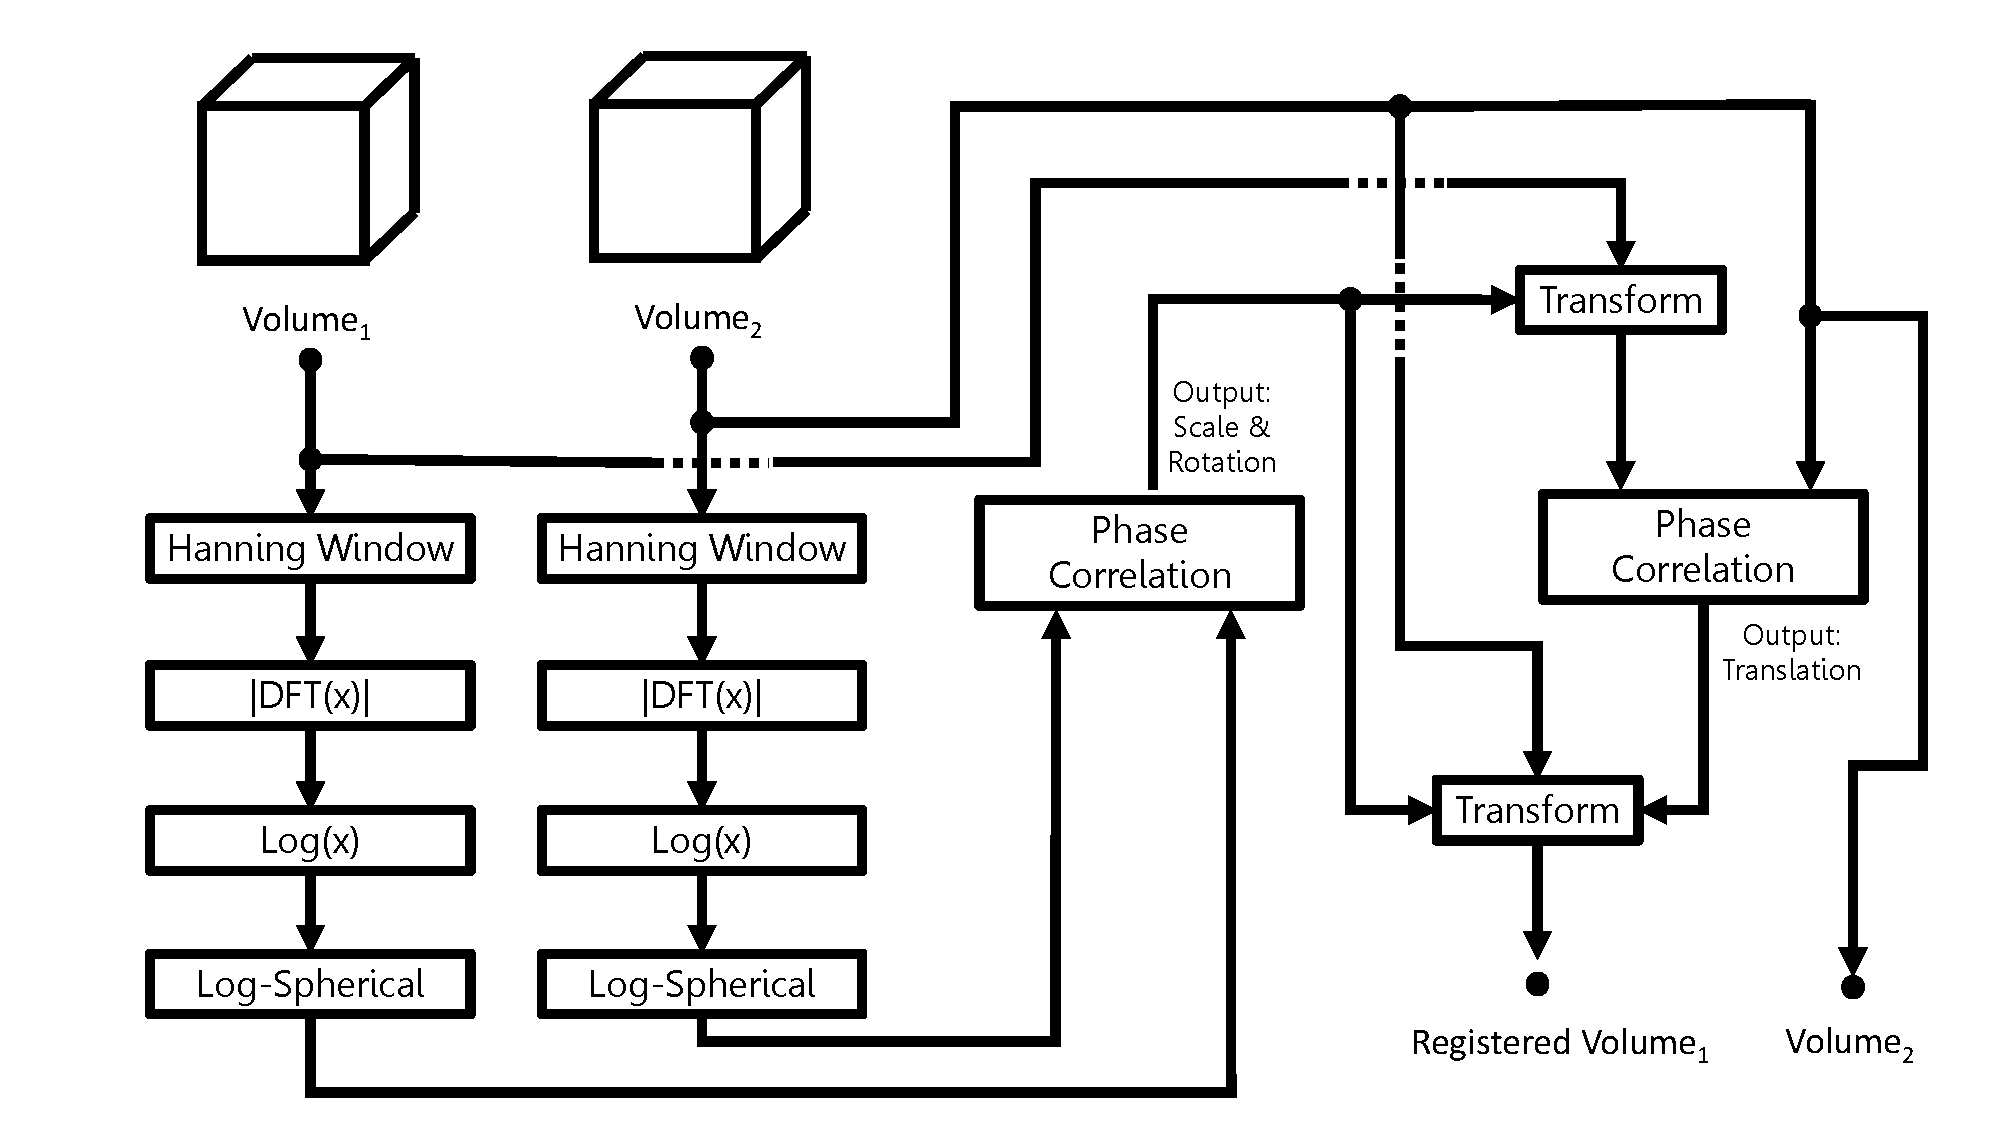
\includegraphics[width=6.0in]{images/ch2/pipeline2}
\caption{System Diagram for Registration Process}
\label{fig:PIPELINE}
\end{figure*}


\subsection{Error metrics}

\label{metricsSection}

In order to evaluate the accuracy of volume registration we use several error metrics including: Hausdorff error, mean squared error and the percentage of matched voxels. We describe mathematically those techniques here. All measurements are based on a simple function which computes the nearest neighbour for a given 3D point or voxel given a volume (or collection of 3D points). We define such a function, named nearest-neighbour in equation \ref{eqn:NN}.

\begin{equation} \label{eqn:NN}
NN(p, V) =  \{ q \in V | (Dist(q, p) < Dist(k, p))  \forall k \in V \}
\end{equation}

This function retrieves the closest corresponding point given a query point $p$ and a volume or point cloud of points, $V$. This function can be used to provide omni-directional error functions based on Hausdorff, mean squared and percentage accuracy error metrics.

Here some one-way error functions are described. The one was Hausdorff error is defined in \ref{eqn:HDOW} 

\begin{equation} \label{eqn:HDOW}
\sum_{k=0}^{N} Dist(P_k, NN(P_k, Q))
\end{equation}

\subsection{Reconstruction Integration}

Using the techniques of registration described in the above sections, there are several techniques which may be used to integrate these registered data. In most experiments we use the volume integration to combine the registered data in a single global model. We also propose several techniques for data representation and evaluate their abilities (see section \ref{sec:3DDataRepresentations}). As for the typical volume integration used, we create volumes with dimensions of $512\times 512\times 512$, although larger sizes may be used for increased accuracy. Once a frame is registered, it is projected into the volume. \\

This projection follows the following formula


\begin{equation} \label{eqn:volIntegration}
\begin{split}
x^{1} & = floor((x - frameCenter_x) \times scalar + volumeCenter_x) \\
y^{1} & = floor((y - frameCenter_y) \times scalar + volumeCenter_y) \\
z^{1} & = floor((z - frameCenter_z) \times scalar + volumeCenter_z)
\end{split}
\end{equation}

$frameCenter$ is the center of the projected frame space and $volumeCenter$ is the center of the integration volume, typically scalar is set to 1 or is used to trade-off resolution and map size. An example of an integration process is illustrated in figure XFDF. 


\subsection{Advantages and Disadvantages}



